\documentclass[solution, letterpaper]{cs121}

\usepackage{tikz-qtree}

%% Please fill in your name and collaboration statement here.
%\newcommand{\studentName}{Renzo Lucioni and Daniel Broudy}
%\newcommand{\collaborationStatement}{I collaborated with...}
\newcommand{\solncolor}{red}
\begin{document}

\header{1}{February 15, 2013, at 12:00 PM}{}{}

%%%%%%%%%%%%%%%%%%%%%%%%%%%%%%%%%%%%%%%%%%%%%%%%%%%%
\problem{15}
\subproblem The following are information gain calculations performed by the ID3 algorithm when deciding on which attribute, \emph{A} or \emph{B}, to split. First, we estimate the initial entry before splitting.

\[ H(\text{labels}) \approx \frac{4}{7} (\log_2 \frac{7}{4}) + \frac{3}{7} (\log_2 \frac{7}{3}) \approx 0.99 \]

Next, we calculate the specific conditional entropy of the labels given \emph{A} = 1.

\[ H(\text{labels } | \text{ } A = 1) \approx \frac{1}{2} (\log_2 2) + \frac{1}{2} (\log_2 2) = 1 \]

Then we compute the specific conditional entropy of the labels given \emph{A} = 0.

\[ H(\text{labels } | \text{ } A = 0) \approx \frac{2}{3} (\log_2 \frac{3}{2}) + \frac{1}{3} (\log_2 3) \approx 0.92 \]

Now we find the conditional entropy of the labels given that we split on \emph{A}.

\[ H(\text{labels } | \text{ } A) \approx \frac{4}{7}(1) + \frac{3}{7}(0.92) \approx 0.97 \]

Finally, we estimate the mutual information between \emph{A} and the labels.

\[ I(\text{labels } ; \text{ } A) \approx  0.99 - 0.97 \approx 0.02\]

Using the same procedure, we compute the information gain from splitting on \emph{B}.

\[ H(\text{labels } | \text{ } B = 1) \approx  \frac{1}{2} (\log_2 2) + \frac{1}{2} (\log_2 2) = 1 \]

\[ H(\text{labels } | \text{ } B = 0) \approx  \frac{3}{5} (\log_2 \frac{5}{3}) + \frac{2}{5} (\log_2 \frac{5}{2}) \approx 0.97 \]

\[ H(\text{labels } | \text{ } B) \approx \frac{2}{7}(1) + \frac{5}{7}(0.97) \approx 0.98 \]

\[ I(\text{labels } ; \text{ } B) \approx  0.99 - 0.98 \approx 0.01 \]

Now we compare the possible information gains. Since $0.02 > 0.01$, ID3 will decide to split on attribute \emph{A}.

One can argue that splitting on \emph{A} is more useful than splitting on \emph{B}, since it is the attribute associated with the largest local information gain (i.e., the entropy of the negative value is locally the lowest). However, one can also argue that splitting on \emph{B} is more useful than splitting on \emph{A}, since doing so allows for immediately labeling 3 of 7 instances as positive and giving  ``no information" on 2 instances, whereas splitting on \emph{A} allows for labeling only 2 of 7 instances as positive and giving ``no information" on 4 instances. This example shows that ID3 has a preference for trees with high information gain attributes near the root, simultaneously demonstrating the algorithm's preference for making the most extreme local partition possible.

\subproblem The following is a decision tree ID3 might construct for the given dataset.

\begin{center}
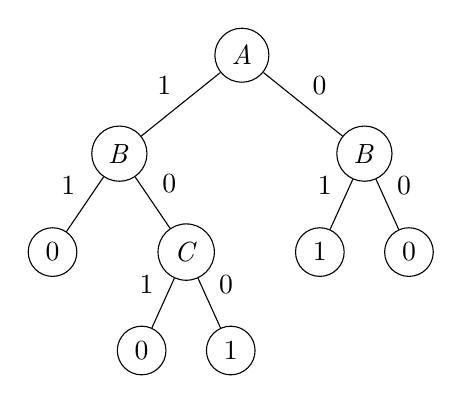
\begin{tikzpicture}[every tree node/.style={draw,circle},
   level distance=1.25cm,sibling distance=.5cm, 
   edge from parent path={(\tikzparentnode) -- (\tikzchildnode)}]
\Tree [.\node {\emph{A}}; 
    \edge node[auto=right] {1}; [.\emph{B}
      \edge node[auto=right] {1}; [.0 ] \edge node[auto=left] {0}; [.\emph{C} 
        \edge node[auto=right] {1}; [.0 ] \edge node[auto=left] {0}; [.1 ] 
      ]
    ]
    \edge node[auto=left] {0}; [.\emph{B}
      \edge node[auto=right] {1}; [.1 ] \edge node[auto=left] {0}; [.0 ]
    ] ]
\end{tikzpicture}
\end{center}

Attribute \emph{A} yields the highest information gain, so ID3 uses \emph{A} as the root of the tree. After arbitrarily breaking an information gain tie with \emph{C}, \emph{B} is chosen as the first node on the left. \emph{C} is chosen as the next node extending from \emph{B} because it fully explains the remaining data. After arbitrarily breaking an information gain tie with \emph{C}, \emph{B} is chosen as the first node on the right. At this point we see that we have inconsistent data but no features left to branch on, so we select the majority target to minimize the number of misclassified examples. The resulting tree misclassifies 1 of 7 examples, indicating that this classifier has an accuracy of $\frac{6}{7} \approx 0.86$.


\subproblem The following is a simpler tree that has the same training error as the one produced by ID3.

\begin{center}
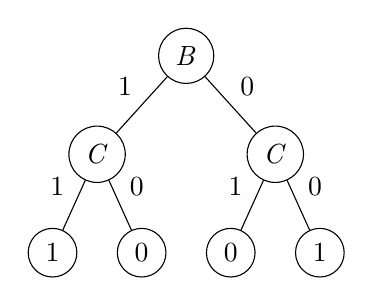
\begin{tikzpicture}[every tree node/.style={draw,circle},
   level distance=1.25cm,sibling distance=.5cm, 
   edge from parent path={(\tikzparentnode) -- (\tikzchildnode)}]
\Tree [.\node {\emph{B}}; 
    \edge node[auto=right] {1}; [.\emph{C}
      \edge node[auto=right] {1}; [.1 ] \edge node[auto=left] {0}; [.0 ]
    ]
    \edge node[auto=left] {0}; [.\emph{C}
      \edge node[auto=right] {1}; [.0 ] \edge node[auto=left] {0}; [.1 ]
    ] ]
\end{tikzpicture}
\end{center}

This tree also has accuracy 0.86. This example shows us that ID3 does not always build the simplest tree possible, but instead finds a ``good" tree which is an approximation of the simplest tree. More importantly, this example also teaches us that ID3 is unable to look ahead to see which attributes are good co-predictors. 

%%%%%%%%%%%%%%%%%%%%%%%%%%%%%%%%%%%%%%%%%%%%%%%%%%%%
\problem{25}
\subproblem The average cross-validated training performance over the ten trials for the non-noisy dataset is 1.0; the test performance is 0.87. The average cross-validated training performance over the ten trials for the noisy dataset is 0.98; the test performance is 0.78.
\pagebreak
\subproblem
 
(i) Graphs of the cross-validated training and test accuracy for both the non-noisy dataset and noisy dataset for validation set sizes in the range [1, 80] have been submitted alongside this document. The graphs are contained in PDF files titled {\tt prune-non-noisy.pdf} and {\tt prune-noisy.pdf}, respectively. \\

(ii) The cross-validated performance (i.e., predictive accuracy) of the validation set pruning increases dramatically as the size of the validation set changes from 1 to 10. The cross-validated performance peaks for validation set sizes of about 20, then decreases gradually as the validation set size approaches 80. \\

(iii) Yes, the validation set pruning improves the cross-validated performance of ID3 on these data. \emph{Without} validation set pruning, the average cross-validated test performance over ten trials for the non-noisy dataset is 0.87 (as stated above). With validation set pruning, the average cross-validated test performance over ten trials for the non-noisy dataset reaches 0.93 when the validation set size is 18 (0.92 training accuracy). For the noisy dataset, the average cross-validated test performance over ten trials improves from 0.78 without pruning to 0.82 with pruning when the validation set size is 11 (0.93 training accuracy). \\

(iv) Yes, overfitting is an issue for these data. The unpruned tree generated in (A) has high average cross-validated training performance over the ten trials on both the noisy and non-noisy datasets. As demonstrated in (iii), while pruning negatively impacts training performance by simplifying the tree, it improves average cross-validated test performance over ten trials for both datasets, suggesting that pruning helps the tree to generalize better. This implies that the original, unpruned tree was overfit.

%%%%%%%%%%%%%%%%%%%%%%%%%%%%%%%%%%%%%%%%%%%%%%%%%%%%
\problem{30}
\subproblem In order to implement boosting, we must define an information gain criterion that takes example weights into account. We can do so by modifying ID3's definition of entropy given weights $w_n^{(r)}$ on the data. More specifically, we will weight the counts of instances in each class by the weight on the instance. We will make a similar change to the method used to compute mutual information in problem (1). Since the problem at hand involves binary classification, making this change allows us to take into account the weights on each training instance by treating the class labels as indicator random variables.

If the weight $w_1 = 0.5$ and the others are $0.5/(N-1)$, then the weighted entropy of the given set is
\[ H(\mathcal D) \approx \frac{.5}{1} (\log_2 \frac{1}{0.5}) + 0 = 0.5 \]

\subproblem

(i) \\

(ii) \\

(iii) \\

(iv) \\


\end{document}



